\chapter{Сценарии диалога (ЛР5)}

% Местозаменитель шаблона фразы: \lrslot{ликёр} печатается как <ликёр>
\newcommand{\lrslot}[1]{$\langle$#1$\rangle$}

\section{Постановка задачи}

Начиная с ЛР5 курс строит диалоговую систему. Пользователь задаёт вопрос на русском языке, а система отвечает или выполняет запрос к рекомендательной системе из ЛР3--ЛР4. Тема диалога остаётся прежней --- ликёры. Поэтому диалоговая система станет новым интерфейсом к уже готовым данным и алгоритмам.

ЛР5 готовит сценарии беседы для такой системы. Требуется:
\begin{itemize}[leftmargin=1.6\parindent, label*=---]
	\item выделить классы вопросов, которые пользователь задаёт на эту тему;
	\item подготовить не менее пяти вопросов каждого класса;
	\item переформулировать каждый вопрос двумя-тремя способами;
	\item определить опорные слова, по которым узнаётся класс вопроса;
	\item записать шаблоны фраз с местозаменителями и расшифровать их;
	\item задать вежливый ответ по шаблону на вопросы, на которые ответить нельзя.
\end{itemize}

Корпус вопросов, словари и проверка хранятся в каталоге \code{5-dialogue} репозитория.

\section{Классы вопросов}

Классы выбраны по тому, какая часть системы должна ответить на вопрос (таблица~\ref{tab:lr5_classes}). Тогда класс вопроса сразу определяет обработчик ответа. Справку о домене даёт датасет ЛР1, подбор выполняют рекомендатель ЛР3 и поиск ЛР4, сравнение опирается на меру близости ЛР2.

\begin{table}[H]
	\centering
	\caption{Классы вопросов диалоговой системы}
	\label{tab:lr5_classes}
	\footnotesize
	\begin{tabular}{|c|L{3.4cm}|L{5.4cm}|L{4.8cm}|}
		\hline
		№ & Класс & Что спрашивают & Источник ответа \\ \hline
		1 & о предметной области & что такое ликёр, крепость, состав, виды ликёров, состав коктейля & датасет ЛР1, таксономия вкуса, база коктейлей \\ \hline
		2 & о функцио\-нальности системы & что система умеет и чего не умеет & справка о возможностях \\ \hline
		3 & поиск и рекомендации & что похоже на ликёр, что найти по условиям, что добавить в кофе или коктейль, с чем смешать & рекомендатель ЛР3, поиск ЛР4, база коктейлей \\ \hline
		4 & сравнение двух объектов & чем один ликёр отличается от другого, что слаще или крепче & мера близости ЛР2 и вклады признаков \\ \hline
		5 & изменение состава системы & добавить, удалить или изменить ликёр, вкусовую группу, коктейль & команды правки данных \\ \hline
		6 & нельзя дать ответ & цены и магазины, погода, дозы алкоголя и здоровье, факты вне базы & вежливый ответ по шаблону \\ \hline
	\end{tabular}
\end{table}

Границы классов проведены по нескольким правилам.
\begin{itemize}[leftmargin=1.6\parindent, label*=---]
	\item \textbf{Коктейли разделены между классами 1 и 3.} Вопрос <<из чего состоит B-52>> просит знание о домене, ответ на него не зависит от вкуса пользователя. Вопросы <<какой ликёр добавить в кофе>>, <<чем заменить Cointreau в Маргарите>> и <<с чем смешать Malibu>> просят подбор. На них отвечает рекомендатель с учётом базы коктейлей.
	\item \textbf{Сравнение выделено в отдельный класс.} В вопросе два конкретных ликёра, а ответ строится по мере близости ЛР2 и её вкладам. Рекомендация, наоборот, отталкивается от одного образца или от ограничений.
	\item \textbf{Вопрос о возможности --- класс 2, а не просьба.} <<Ты умеешь подбирать ликёры?>> спрашивает о системе. Ответ на него --- справка, а не список ликёров.
	\item \textbf{Класс 6 включает вопросы о дозах алкоголя и о здоровье.} Данные для них в системе есть только частично, например крепость. Совет о том, сколько можно выпить или можно ли пить при болезни, рекомендательная система давать не должна.
\end{itemize}

Для вопросов о коктейлях подготовлена база \code{cocktails.json}. В ней девять коктейлей с ликёрами каталога, например B-52, Белый русский, Эспрессо-мартини, Маргарита и Кузнечик. Там же указаны миксеры, с которыми ликёры обычно смешивают, например Malibu с ананасовым соком, Fernet-Branca с колой и Kahl\'ua с молоком. Ликёры в базе указаны идентификаторами датасета, поэтому подбор замены в коктейле может использовать меру близости ЛР2.

На рисунке~\ref{fig:lr5_flow} показано, как вопрос будет проходить через диалоговую систему. ЛР5 реализует левую часть схемы до выбора класса. Обработчики классов строятся в следующих работах.

\begin{figure}[H]
	\centering
	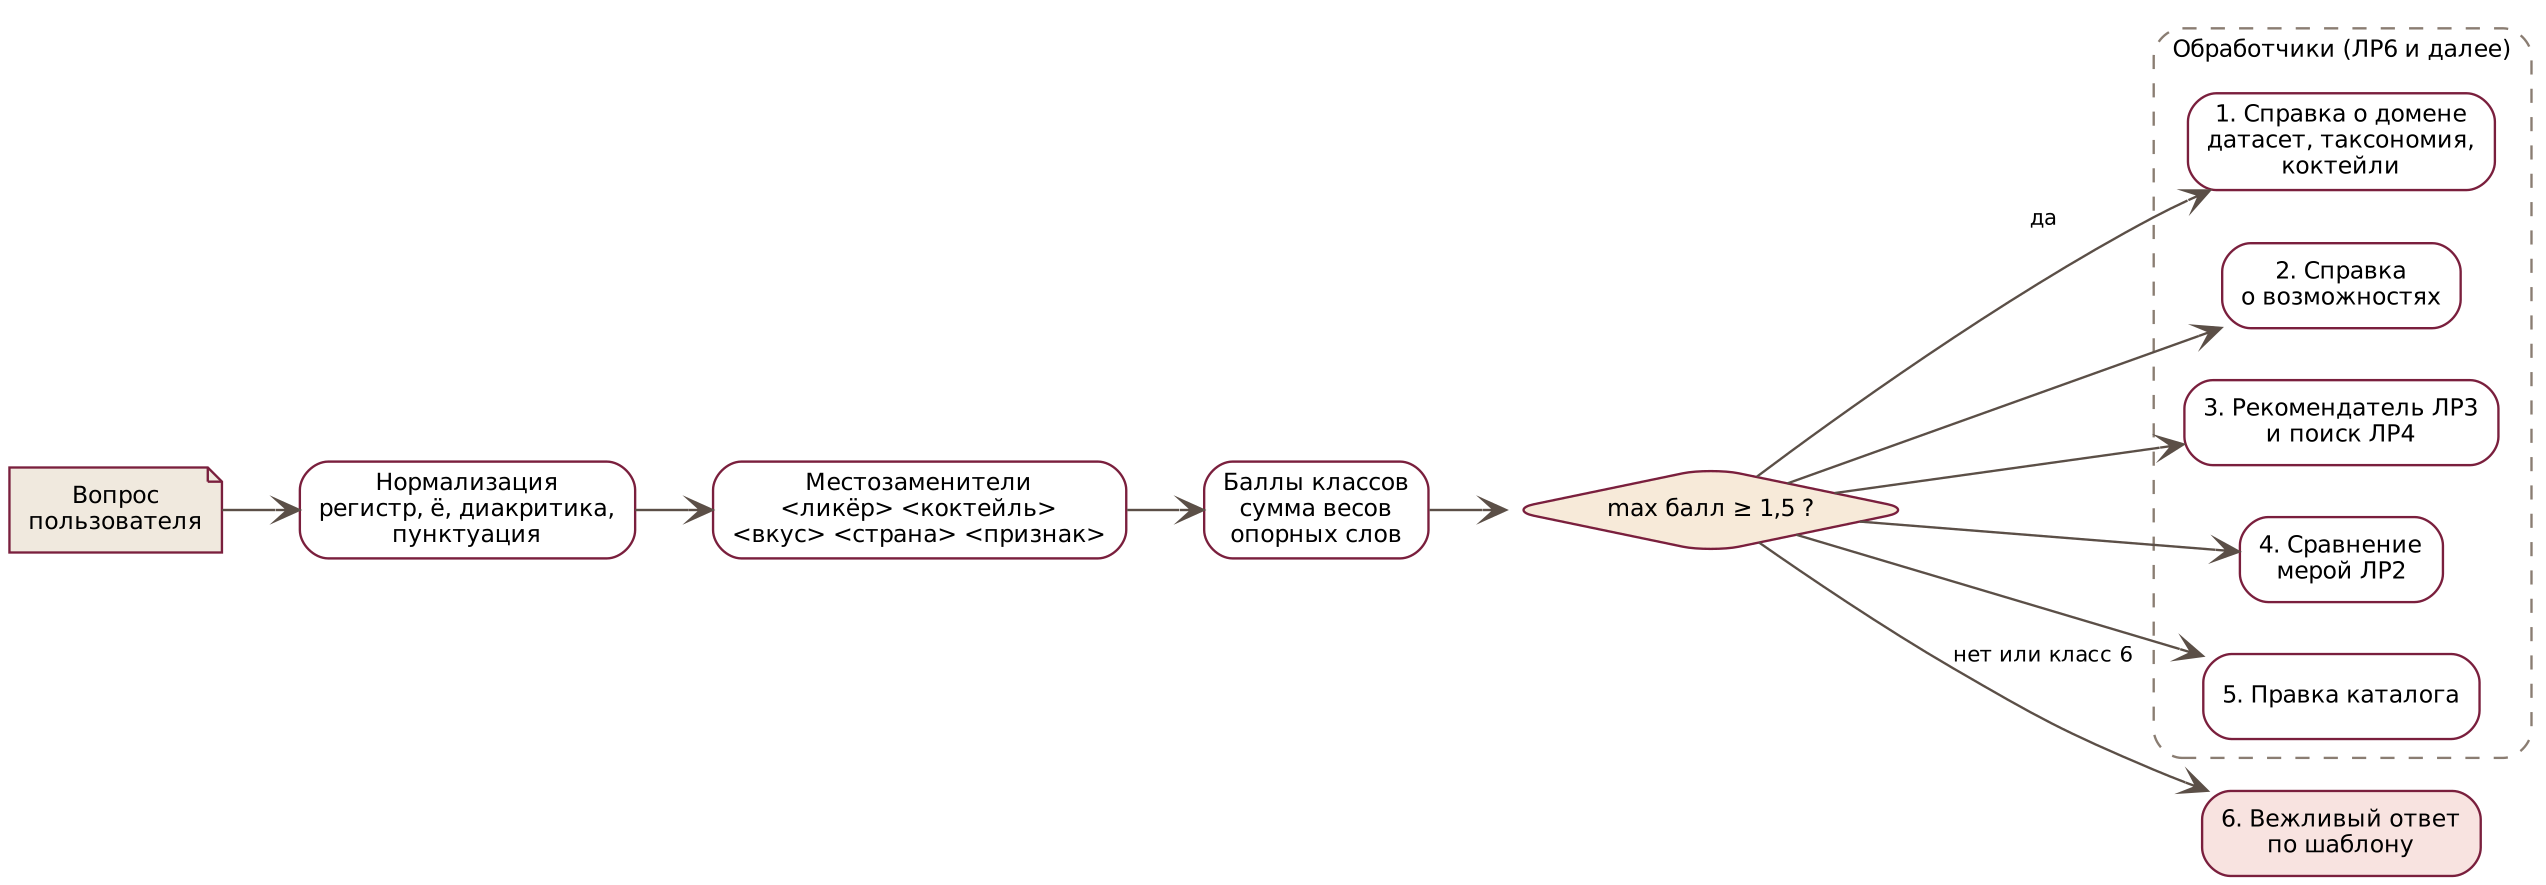
\includegraphics[width=\textwidth]{diags/dialogue.png}
	\caption{Обработка вопроса: от текста к классу и обработчику}
	\label{fig:lr5_flow}
\end{figure}

\section{Вопросы и переформулировки}

Корпус содержит 37 исходных вопросов, от шести до семи в каждом классе, и по три переформулировки каждого вопроса. Всего 148 формулировок (таблицы~\ref{tab:lr5_class1}--\ref{tab:lr5_class6}). Переформулировки построены несколькими способами, чтобы проверить разные явления живой речи:
\begin{itemize}[leftmargin=1.6\parindent, label*=---]
	\item замена вопросительного слова и порядка слов: <<Какая крепость у J\"agermeister?>> и <<Насколько крепкий J\"agermeister?>>;
	\item синонимы и близкие глаголы: <<посоветуй>>, <<подбери>>, <<найди>>, <<что ещё попробовать>>;
	\item разное написание названий: Baileys и Бейлиз, J\"agermeister, Егермейстер и Егерь;
	\item разговорные и неполные фразы: <<Фернет нравится, J\"agermeister нет --- подбери что-нибудь>>;
	\item перенос смысла в другую часть речи: <<сравни сладость>> вместо <<что слаще>>.
\end{itemize}

\subsection{Класс 1. Вопросы о предметной области}

{\renewcommand{\arraystretch}{0.85}
\begin{longtable}{|F{0.9cm}|F{5.6cm}|F{8.2cm}|}
	\caption{Вопросы класса 1 и их переформулировки}\label{tab:lr5_class1}\\ \hline
	№ & Вопрос & Переформулировки \\ \hline
	\endfirsthead
	\multicolumn{3}{l}{Продолжение таблицы~\ref{tab:lr5_class1}} \\ \hline
	№ & Вопрос & Переформулировки \\ \hline
	\endhead
	1.1 & Что такое ликёр? & --- Чем ликёр отличается от обычного крепкого алкоголя? \newline --- Объясни, что называют ликёром. \newline --- Какой напиток можно назвать ликёром? \\ \hline
	1.2 & Какая крепость у J\"agermeister? & --- Сколько градусов в Егермейстере? \newline --- Насколько крепкий J\"agermeister? \newline --- Подскажи процент алкоголя в J\"agermeister. \\ \hline
	1.3 & Какие бывают виды ликёров по вкусу? & --- На какие группы делятся ликёры? \newline --- Какие вкусовые категории ликёров ты знаешь? \newline --- Перечисли типы ликёров. \\ \hline
	1.4 & Из чего делают Baileys? & --- На какой основе сделан Бейлиз? \newline --- Что входит в состав Baileys? \newline --- Baileys --- это ликёр на чём? \\ \hline
	1.5 & Что такое амаро? & --- Какие ликёры относятся к амаро? \newline --- Расскажи про категорию амаро. \newline --- Чем характерны амаро? \\ \hline
	1.6 & Какие ликёры входят в коктейль B-52? & --- Из каких ликёров состоит Б-52? \newline --- Что нужно для коктейля Б-52? \newline --- Какой состав у шота B-52? \\ \hline
\end{longtable}
}

\subsection{Класс 2. Вопросы о функциональности системы}

{\renewcommand{\arraystretch}{0.85}
\begin{longtable}{|F{0.9cm}|F{5.6cm}|F{8.2cm}|}
	\caption{Вопросы класса 2 и их переформулировки}\label{tab:lr5_class2}\\ \hline
	№ & Вопрос & Переформулировки \\ \hline
	\endfirsthead
	\multicolumn{3}{l}{Продолжение таблицы~\ref{tab:lr5_class2}} \\ \hline
	№ & Вопрос & Переформулировки \\ \hline
	\endhead
	2.1 & Что ты умеешь? & --- Какие у тебя функции? \newline --- Чем ты можешь мне помочь? \newline --- Что можно у тебя спросить? \\ \hline
	2.2 & Ты можешь подобрать ликёр по моим предпочтениям? & --- Ты умеешь давать рекомендации? \newline --- Умеешь советовать ликёры по вкусу? \newline --- Ты рекомендуешь напитки по лайкам? \\ \hline
	2.3 & Ты можешь заказать мне бутылку? & --- Умеешь ли ты оформлять покупки? \newline --- Можно через тебя купить ликёр? \newline --- Ты продаёшь ликёры? \\ \hline
	2.4 & Сколько ликёров есть в твоей базе? & --- Какой у тебя каталог? \newline --- Со сколькими ликёрами ты работаешь? \newline --- Насколько большая у тебя база ликёров? \\ \hline
	2.5 & По каким параметрам можно искать? & --- Какие фильтры поиска ты поддерживаешь? \newline --- По каким признакам ты ищешь ликёры? \newline --- Что можно указать в запросе на поиск? \\ \hline
	2.6 & Как ты учитываешь мои дизлайки? & --- Что ты делаешь с ликёрами, которые мне не понравились? \newline --- Как дизлайки влияют на твои советы? \newline --- Зачем тебе знать, что мне не нравится? \\ \hline
\end{longtable}
}

\subsection{Класс 3. Вопросы на поиск и рекомендации}

{\renewcommand{\arraystretch}{0.85}
\begin{longtable}{|F{0.9cm}|F{5.6cm}|F{8.2cm}|}
	\caption{Вопросы класса 3 и их переформулировки}\label{tab:lr5_class3}\\ \hline
	№ & Вопрос & Переформулировки \\ \hline
	\endfirsthead
	\multicolumn{3}{l}{Продолжение таблицы~\ref{tab:lr5_class3}} \\ \hline
	№ & Вопрос & Переформулировки \\ \hline
	\endhead
	3.1 & Посоветуй что-нибудь похожее на Baileys. & --- Что ещё мне может понравиться, если я люблю Бейлиз? \newline --- Найди ликёр в стиле Baileys. \newline --- Какой ликёр похож на Baileys? \\ \hline
	3.2 & Найди травяной ликёр крепче 30 градусов. & --- Покажи травяные ликёры от 30 \%. \newline --- Есть ли травяной ликёр крепостью больше 30? \newline --- Хочу травяной ликёр не слабее 30 градусов. \\ \hline
	3.3 & Подбери сладкий ликёр из Италии. & --- Какие сладкие итальянские ликёры есть? \newline --- Покажи итальянские ликёры с высоким содержанием сахара. \newline --- Хочу что-нибудь сладкое итальянское. \\ \hline
	3.4 & Мне понравился Fernet-Branca, но не понравился J\"agermeister. Что посоветуешь? & --- Люблю Фернет, а Егермейстер не нравится. Что ещё попробовать? \newline --- Фернет нравится, J\"agermeister нет --- подбери что-нибудь. \newline --- Что выбрать, если Fernet понравился, а Егерь нет? \\ \hline
	3.5 & Какой ликёр добавить в кофе? & --- Что подлить в кофе из ликёров? \newline --- Посоветуй ликёр к кофе. \newline --- Какой ликёр подойдёт для кофе? \\ \hline
	3.6 & Чем заменить Cointreau в Маргарите? & --- Что можно взять вместо Куантро для Маргариты? \newline --- Какой ликёр подойдёт в Маргариту, если нет Cointreau? \newline --- Нет Куантро, что положить в Маргариту? \\ \hline
	3.7 & С чем смешать Malibu? & --- С чем пить Малибу? \newline --- Что миксовать с Malibu? \newline --- С каким соком сочетается Malibu? \\ \hline
\end{longtable}
}

\subsection{Класс 4. Вопросы на сравнение двух объектов}

{\renewcommand{\arraystretch}{0.85}
\begin{longtable}{|F{0.9cm}|F{5.6cm}|F{8.2cm}|}
	\caption{Вопросы класса 4 и их переформулировки}\label{tab:lr5_class4}\\ \hline
	№ & Вопрос & Переформулировки \\ \hline
	\endfirsthead
	\multicolumn{3}{l}{Продолжение таблицы~\ref{tab:lr5_class4}} \\ \hline
	№ & Вопрос & Переформулировки \\ \hline
	\endhead
	4.1 & Чем Cointreau отличается от Grand Marnier? & --- В чём разница между Куантро и Гран Марнье? \newline --- Cointreau или Grand Marnier: какой взять? \newline --- Сравни Cointreau и Grand Marnier. \\ \hline
	4.2 & Что слаще: Baileys или Amarula? & --- Какой из них слаще, Бейлиз или Амарула? \newline --- В каком больше сахара, Baileys или Amarula? \newline --- Сравни сладость Baileys и Amarula. \\ \hline
	4.3 & Насколько похожи J\"agermeister и Fernet-Branca? & --- Похож ли Егермейстер на Фернет? \newline --- Близки ли J\"agermeister и Fernet по вкусу? \newline --- Насколько Fernet-Branca похож на J\"agermeister? \\ \hline
	4.4 & Какой крепче: Chartreuse Verte или G\'en\'epi? & --- Что крепче, Шартрез или Женепи? \newline --- В каком больше градусов, Chartreuse или G\'en\'epi? \newline --- Сравни крепость Шартреза и Женепи. \\ \hline
	4.5 & Disaronno и Luxardo Amaretto --- это одно и то же? & --- Есть ли разница между Дисаронно и Луксардо Амаретто? \newline --- Disaronno и Luxardo одинаковые? \newline --- Отличается ли Disaronno от Luxardo Amaretto? \\ \hline
	4.6 & Kahl\'ua или Mr Black: что лучше для эспрессо-мартини? & --- Для эспрессо-мартини лучше Калуа или Мистер Блэк? \newline --- Что выбрать в эспрессо-мартини: Kahl\'ua или Mr Black? \newline --- Сравни Kahl\'ua и Mr Black для эспрессо-мартини. \\ \hline
\end{longtable}
}

\subsection{Класс 5. Вопросы на изменение состава системы}

{\renewcommand{\arraystretch}{0.85}
\begin{longtable}{|F{0.9cm}|F{5.6cm}|F{8.2cm}|}
	\caption{Вопросы класса 5 и их переформулировки}\label{tab:lr5_class5}\\ \hline
	№ & Вопрос & Переформулировки \\ \hline
	\endfirsthead
	\multicolumn{3}{l}{Продолжение таблицы~\ref{tab:lr5_class5}} \\ \hline
	№ & Вопрос & Переформулировки \\ \hline
	\endhead
	5.1 & Добавь в каталог ликёр Aperol. & --- Внеси Aperol в базу. \newline --- Хочу добавить новый ликёр Aperol. \newline --- Запиши Апероль в список ликёров. \\ \hline
	5.2 & Удали Midori из базы. & --- Убери Мидори из каталога. \newline --- Исключи Midori из списка ликёров. \newline --- Midori больше не нужен в базе, сотри его. \\ \hline
	5.3 & Измени крепость Kahl\'ua на 20 \%. & --- Поправь крепость Калуа: 20 градусов. \newline --- У Kahl\'ua теперь 20 \%, обнови данные. \newline --- Установи для Kahl\'ua крепость 20. \\ \hline
	5.4 & Отметь, что Frangelico выдерживается в дереве. & --- У Frangelico есть контакт с деревом, исправь. \newline --- Поставь Франжелико признак выдержки в дереве. \newline --- Frangelico выдерживают в бочке, учти это. \\ \hline
	5.5 & Добавь в таксономию новую вкусовую группу <<Медовые>>. & --- Создай вкусовую категорию <<Медовые>>. \newline --- Нужна новая ветка <<Медовые>> в классификации вкусов. \newline --- Заведи группу вкуса <<Медовые>>. \\ \hline
	5.6 & Добавь коктейль Mudslide: водка, Kahl\'ua и Baileys. & --- Запомни новый коктейль Mudslide с Калуа и Бейлиз. \newline --- Внеси рецепт Mudslide в базу коктейлей. \newline --- Сохрани коктейль Mudslide из Kahl\'ua, Baileys и водки. \\ \hline
\end{longtable}
}

\subsection{Класс 6. Вопросы, на которые нельзя дать ответ}

{\renewcommand{\arraystretch}{0.85}
\begin{longtable}{|F{0.9cm}|F{5.6cm}|F{8.2cm}|}
	\caption{Вопросы класса 6 и их переформулировки}\label{tab:lr5_class6}\\ \hline
	№ & Вопрос & Переформулировки \\ \hline
	\endfirsthead
	\multicolumn{3}{l}{Продолжение таблицы~\ref{tab:lr5_class6}} \\ \hline
	№ & Вопрос & Переформулировки \\ \hline
	\endhead
	6.1 & Сколько стоит Baileys? & --- Какая цена у Бейлиз? \newline --- Почём сейчас Baileys? \newline --- Сколько рублей за бутылку Baileys? \\ \hline
	6.2 & Где купить Chartreuse в Москве? & --- В каком магазине продаётся Шартрез? \newline --- Где найти Chartreuse поблизости? \newline --- Подскажи, где взять Шартрез в Москве. \\ \hline
	6.3 & Какая завтра погода? & --- Будет ли завтра дождь? \newline --- Сколько градусов будет завтра на улице? \newline --- Что с погодой на выходных? \\ \hline
	6.4 & Сколько ликёра можно выпить, чтобы не опьянеть? & --- Сколько рюмок можно выпить и сесть за руль? \newline --- Какая доза ликёра безопасна? \newline --- Сколько J\"agermeister выпить, чтобы не было похмелья? \\ \hline
	6.5 & Можно ли пить ликёр при простуде? & --- Совместим ли Baileys с антибиотиками? \newline --- Можно ли ликёр при больном горле? \newline --- Помогает ли Fernet от простуды? \\ \hline
	6.6 & Какой ликёр пил Хемингуэй? & --- Какой ликёр любил Хемингуэй? \newline --- Что из ликёров предпочитал Хемингуэй? \newline --- Хемингуэй пил какой ликёр? \\ \hline
\end{longtable}
}


\section{Местозаменители и шаблоны фраз}

Многие вопросы различаются только названием ликёра, вкуса или числом. Такие места шаблона заменены местозаменителями (таблица~\ref{tab:lr5_slots}). Их значения хранятся в словаре \code{lexicon.json}. Для каждого ликёра записаны оригинальное название и русские написания, потому что пользователь пишет и <<Baileys>>, и <<Бейлиз>>. Значения хранятся основами. Основа <<шартрез>> находит и <<Шартрез>>, и <<Шартреза>>, поэтому склонение не мешает поиску.

\begin{table}[H]
	\centering
	\caption{Местозаменители шаблонов фраз}
	\label{tab:lr5_slots}
	\footnotesize
	\begin{tabular}{|L{3.4cm}|L{11.6cm}|}
		\hline
		Местозаменитель & Значения \\ \hline
		\lrslot{ликёр} & 30 ликёров каталога и их написания: Baileys, Бейлиз, Бейлис; J\"agermeister, Егермейстер, Егерь; Cointreau, Куантро и т.\,д. \\ \hline
		\lrslot{коктейль} & B-52, Белый русский, Эспрессо-мартини, Mudslide, Маргарита, Космополитен, Кузнечик, Кир, Амаретто сауэр \\ \hline
		\lrslot{вкус} & узлы таксономии ЛР1: травяной, фруктовый, цитрусовый, ягодный, сливочный, кофейный, амаро, кройтер и др. \\ \hline
		\lrslot{страна} & страна и прилагательное от неё: Италия, итальянский; Франция, французский и др. \\ \hline
		\lrslot{признак} & крепость, градус; сахар, сладость; объём; горечь; дерево, бочка, выдержка \\ \hline
		\lrslot{число} & число с единицей измерения: \%, градусов, г/л, л \\ \hline
		ge & больше | крепче | выше | от | не меньше | не слабее \\ \hline
		le & меньше | слабее | ниже | до | не больше | не крепче \\ \hline
		сравн & слаще | крепче | горче | лучше \\ \hline
	\end{tabular}
\end{table}

Шаблоны записаны в нотации регулярных выражений, как в методических указаниях~\cite{friedl2008}. Квадратные скобки обозначают выбор одного варианта, фигурные --- выбор из множества местозаменителей, знак <<?>> после скобки --- необязательную часть.

{\footnotesize
\begin{verbatim}
1: [что такое | расскажи про | что называют] {<вкус>|<ликёр>|ликёр} ?
   [какая крепость у | сколько градусов в | насколько крепкий] <ликёр> ?
   [из чего делают | что входит в состав | из каких ликёров состоит]
       {<ликёр>|<коктейль>} ?
2: [что | как] ты [умеешь | можешь | учитываешь] ...?
   [по каким параметрам | какие фильтры] [можно искать | ты поддерживаешь] ?
3: [посоветуй | найди | подбери | хочу] [что-нибудь]
       [похожее на <ликёр> | <вкус> {ge|le} <число> | из <страна>] .
   [какой ликёр | что] [добавить | подлить] [в | к] {кофе|<коктейль>} ?
   [чем заменить | что взять вместо] <ликёр> в <коктейль> ?
   с чем [смешать | пить | миксовать] <ликёр> ?
4: [чем | в чём разница между] <ликёр> [и | от] <ликёр> ?
   [что | какой] {сравн} [:] <ликёр> или <ликёр> ?
   [сравни] (<признак>)? <ликёр> и <ликёр> .
5: [добавь | внеси | удали | убери | измени | отметь | создай]
       {<ликёр>|<вкус>|<коктейль>} [в | из] [каталог | базу | таксономию]
       ([<признак> на <число>])? .
6: вопросы с маркерами цены, магазина, погоды, дозы и здоровья,
   а также вопросы без опорных слов других классов
\end{verbatim}
}

\section{Опорные слова}

Класс вопроса определяется по опорным словам. Это основы слов и словосочетания, характерные для класса, а также условия на число местозаменителей в вопросе. Каждому опорному слову приписан вес. Класс $c$ получает балл
\begin{equation}
	B_c(q) = \sum_{k} w_{ck}\,[\text{правило } k \text{ класса } c \text{ сработало на } q],
	\label{eq:lr5_score}
\end{equation}
и вопрос относится к классу с наибольшим баллом. Если наибольший балл меньше порога $1{,}5$, вопрос относится к классу 6. Порог равен весу одного слабого признака класса, например упоминания крепости в вопросе о домене. Ниже порога остаются вопросы, в которых нет ни одного уверенного признака известного класса. При равенстве баллов выигрывает класс с более специфичными опорными словами. Порядок проверки такой: функциональность, нельзя ответить, изменение, сравнение, рекомендации, домен. Итоговые опорные слова приведены в таблице~\ref{tab:lr5_keywords}.

\begin{table}[H]
	\centering
	\caption{Опорные слова классов. В скобках --- вес}
	\label{tab:lr5_keywords}
	\footnotesize
	\begin{tabular}{|L{3.3cm}|L{11.7cm}|}
		\hline
		Класс & Опорные слова и условия \\ \hline
		1. домен & что такое, расскажи, объясни, назвать (2); из чего, состав, состоит, основа, на чём, нужно для (2); виды, бывают, типы, категории, группы (3); входит, относится (1,5); отличается, разница (1,5); алкоголь, напиток (1); какая крепость, сколько градусов (1,5); есть \lrslot{коктейль} (1) \\ \hline
		2. функцио\-нальность & ты, тебя, твой (1,5); глагол 2-го лица на -ешь, -ишь (1); умеешь, можешь (2); функции, помочь, зачем, как ты (1,5); параметры, фильтры, по каким, на поиск (2); лайки, учитываешь (2); твоя база, сколько ликёров (2) \\ \hline
		3. поиск и рекомендации & посоветуй, подбери, найди, покажи, хочу, есть ли, что ещё (2); похоже на, в стиле (2); нравится, люблю (2); выбрать (1,5); добавить в, подлить, положить, в кофе (2); заменить, вместо (2,5); смешать, миксовать, сочетается, подойдёт (2,5); ge или le и число (1,5); есть \lrslot{признак} (1); есть \lrslot{вкус} или \lrslot{страна} (0,5) \\ \hline
		4. сравнение & два \lrslot{ликёр} в вопросе (3); сравни, отличается, разница, одно и то же, похожи вместе с \lrslot{ликёр} (2,5); слаще, крепче, горче, лучше (1); или (1) \\ \hline
		5. изменение состава & повелительные глаголы правки: добавь, внеси, удали, убери, измени, обнови, отметь, исправь, создай, заведи, сохрани и др. (3); неопределённая форма этих глаголов (1,5); в каталог, из базы, в таксономию (1,5); новый, теперь (1) \\ \hline
		6. нельзя ответить & стоит, цена, почём, рублей (3); купить, магазин, продаётся, где взять (3); погода, дождь, завтра, на улице (3); выпить, опьянеть, руль, доза, похмелье (3); лекарства, простуда, горло, здоровье (3); отсутствие опорных слов других классов \\ \hline
	\end{tabular}
\end{table}

Принятые решения по опорным словам:
\begin{itemize}[leftmargin=1.6\parindent, label*=---]
	\item \textbf{Основы вместо полных слов.} Русские слова склоняются и спрягаются. Основа <<сравн>> покрывает <<сравни>>, <<сравнить>>, <<сравнение>>. Лемматизация морфологическим анализатором вроде pymorphy2 точнее, но требует внешней библиотеки. Проверка в разделе~\ref{sec:lr5_check} показала, что основ достаточно для различения классов.
	\item \textbf{Местозаменители --- тоже опорные признаки.} Два ликёра в одном вопросе почти всегда означают сравнение, поэтому это условие весит 3. Упоминание страны или вкуса встречается во всех классах, поэтому весит всего 0,5.
	\item \textbf{Обращение к системе отличает класс 2.} Местоимения <<ты>>, <<тебя>> и глаголы 2-го лица на -ешь, -ишь показывают, что пользователь спрашивает о самой системе. Это морфологический признак, а не список глаголов, поэтому он сработает и на глаголах, которых нет в корпусе.
	\item \textbf{Повелительное наклонение отличает класс 5.} Глаголы <<добавь>>, <<удали>>, <<измени>> --- команды. Неопределённая форма весит меньше, потому что <<какой ликёр добавить в кофе>> --- это просьба о подборе, а не команда изменить каталог.
	\item \textbf{Слова сравнения работают только вместе с ликёром.} <<Чем ликёр отличается от крепкого алкоголя>> --- вопрос о домене, а не сравнение двух объектов. Поэтому правило <<отличается>> класса 4 срабатывает, только если в вопросе есть хотя бы один \lrslot{ликёр}.
	\item \textbf{Маркеры класса 6 весят больше всех.} Слова цены, погоды и здоровья однозначно показывают, что ответа в базе нет. Если на вопрос <<Сколько стоит Baileys?>> отвечать как на вопрос о домене, получится справка о крепости Baileys вместо честного <<цен в базе нет>>.
\end{itemize}

\section{Вежливый ответ по шаблону}

На вопросы класса 6 система отвечает по шаблону <<\textit{извинение} + \textit{причина} + \textit{что система может предложить}>>. Причина выбирается по тем же опорным словам (таблица~\ref{tab:lr5_refusals}). Ответ не обрывает разговор. Он объясняет, почему ответа нет, и предлагает вопрос, на который система ответит.

\begin{table}[H]
	\centering
	\caption{Вежливые ответы на вопросы, на которые нельзя ответить}
	\label{tab:lr5_refusals}
	\footnotesize
	\begin{tabular}{|L{2.4cm}|L{3.6cm}|L{9.0cm}|}
		\hline
		Причина & Пример вопроса & Ответ \\ \hline
		нет цен и магазинов & Сколько стоит Baileys? & Извините, в моей базе нет цен и сведений о магазинах. Я могу рассказать о вкусе, крепости и сладости этого ликёра или подобрать похожий. \\ \hline
		вне темы & Какая завтра погода? & Извините, я отвечаю только на вопросы о ликёрах. Спросите, например: <<Посоветуй что-нибудь похожее на Baileys>>. \\ \hline
		здоровье и дозы & Сколько ликёра можно выпить, чтобы не опьянеть? & Извините, я не даю советов о количестве алкоголя и о том, как он сочетается с лекарствами и здоровьем. С такими вопросами лучше обратиться к врачу. Я могу рассказать о крепости, сладости и вкусе ликёров. \\ \hline
		нет сведений & Какой ликёр пил Хемингуэй? & Извините, таких сведений нет в моей базе, поэтому ответить я не могу. Я знаю вкус, крепость, сладость и состав коктейлей для 30 ликёров каталога и могу подобрать ликёр по вашему вкусу. \\ \hline
	\end{tabular}
\end{table}

Вопрос о Хемингуэе показывает, зачем нужна причина по умолчанию. В нём есть слово <\lrslot{ликёр}>, но нет ни одного опорного слова другого класса, и балл не достигает порога. Система не знает ответа и честно говорит об этом.

\section{Проверка опорных слов}
\label{sec:lr5_check}

Опорные слова нужно проверить: по ним должен правильно определяться класс не только исходных вопросов, но и новых формулировок. Для проверки реализован классификатор по формуле~\eqref{eq:lr5_score}. Он прогоняет все формулировки корпуса и сравнивает найденный класс с эталонным. Проверка шла в две итерации.
\begin{enumerate}[leftmargin=1.6\parindent]
	\item \textbf{Первая итерация.} Опорные слова составлены только по 37 исходным вопросам. Переформулировки для неё --- новые фразы. Поэтому точность на них показывает, насколько опорные слова переносятся на другие формулировки.
	\item \textbf{Вторая итерация.} Ошибки первой итерации показали, каких слов не хватает. Добавлены глаголы 2-го лица (<<рекомендуешь>>, <<продаёшь>>), слова состава (<<состоит>>, <<нужно для>>), связка слов сравнения с упоминанием ликёра и неопределённая форма глаголов правки. Эти опорные слова уже настроены с учётом переформулировок.
\end{enumerate}
После настройки написаны 12 контрольных фраз, по две на класс. В настройке они не участвовали, поэтому показывают поведение на действительно новых вопросах. Результаты приведены в таблице~\ref{tab:lr5_check}.

\begin{table}[H]
	\centering
	\caption{Доля правильно классифицированных формулировок}
	\label{tab:lr5_check}
	\footnotesize
	\begin{tabular}{|L{6.2cm}|c|c|}
		\hline
		Набор формулировок & Первая итерация & Итоговые опорные слова \\ \hline
		исходные вопросы & 37/37 & 37/37 \\ \hline
		переформулировки & 95/111 & 110/111 \\ \hline
		контрольные фразы & 10/12 & 11/12 \\ \hline
	\end{tabular}
\end{table}

Первая итерация верно классифицировала 86\,\% переформулировок. Больше всего ошибок пришлось на класс 2: 11 из 18. Вопросы о возможностях системы часто не содержат слов <<умеешь>> или <<можешь>>, например <<Ты продаёшь ликёры?>> или <<Со сколькими ликёрами ты работаешь?>>. Их узнаёт признак глагола 2-го лица, добавленный во второй итерации. Итоговые опорные слова ошибаются на одной переформулировке и одной контрольной фразе (таблица~\ref{tab:lr5_confusion}).
\begin{itemize}[leftmargin=1.6\parindent, label*=---]
	\item <<Можно через тебя купить ликёр?>> отнесён к классу 6 вместо класса 2. Слово <<купить>> весит больше местоимения <<тебя>>. Опорные слова не показывают, кто совершает действие. Различить <<купить через систему>> и <<купить в магазине>> поможет синтаксический разбор, который понадобится в следующих работах.
	\item <<Поменяй страну у Amarula на ЮАР>> отнесён к классу 6 вместо класса 5. Глагола <<поменяй>> нет в списке опорных слов. Словарь синонимов глаголов правки нужно пополнять по мере появления новых формулировок.
\end{itemize}

\begin{table}[H]
	\centering
	\caption{Матрица ошибок итоговых опорных слов на всех 160 формулировках. Строки --- эталонный класс, столбцы --- найденный}
	\label{tab:lr5_confusion}
	\footnotesize
	\begin{tabular}{|l|c|c|c|c|c|c|}
		\hline
		Класс & 1 & 2 & 3 & 4 & 5 & 6 \\ \hline
		1. домен & 26 & 0 & 0 & 0 & 0 & 0 \\ \hline
		2. функцио\-нальность & 0 & 25 & 0 & 0 & 0 & 1 \\ \hline
		3. поиск и рекомендации & 0 & 0 & 30 & 0 & 0 & 0 \\ \hline
		4. сравнение & 0 & 0 & 0 & 26 & 0 & 0 \\ \hline
		5. изменение состава & 0 & 0 & 0 & 0 & 25 & 1 \\ \hline
		6. нельзя ответить & 0 & 0 & 0 & 0 & 0 & 26 \\ \hline
	\end{tabular}
\end{table}

Обе ошибки уходят в класс 6. Это безопасное направление ошибки: система не выполнит лишнюю команду и не выдаст неверную справку, а вежливо скажет, что не поняла вопрос. Ошибок между классами 1--5 нет.

\section*{Выводы}
\addcontentsline{toc}{section}{Выводы}

Для диалоговой системы о ликёрах выделены шесть классов вопросов по тому, какая часть системы на них отвечает. Подготовлены 37 вопросов, от шести до семи в классе, и по три переформулировки каждого. Вопросы о коктейлях разделены между справкой о домене и подбором. Для них составлена база из девяти коктейлей и миксеров. Записаны местозаменители и шаблоны фраз, опорные слова с весами и шаблон вежливого ответа с четырьмя причинами отказа. Проверка показала, что опорные слова верно определяют класс 147 из 148 формулировок корпуса и 11 из 12 новых фраз. Оставшиеся ошибки уходят в безопасный класс 6 и указывают, что дальше понадобятся синтаксический разбор и пополнение словаря синонимов.
